%\documentclass{article}
\documentclass{NSTExam}
\showanswerstrue
\noversion

%\documentclass{article}
\usepackage[utf8]{inputenc}
\usepackage{amsmath}
\usepackage{bbm}
\usepackage{xcolor}
\usepackage{afterpage}
\usepackage{tikz}
\usepackage[compat=1.0.0]{tikz-feynman}
%\usepackage{tikz-feynman}
\usepackage{hyperref}


\newcommand\fra{\frac{|\vec p|}{E+m}}
\newcommand\expi{e^{i\phi}}

\newcommand\hide[1]{{}}


\newcommand\alig[1]{{\begin{align}#1\end{align}}}
\newcommand\com[2]{{
\left[#1,#2\right]
}}
\newcommand\anticom[2]{{
\left\{#1,#2\right\}
}}
\newcommand\unit{
\mathbbm{1}
}
\newcommand\matTwoTwo[4]{
\left(\begin{array}{cc}
#1 & #2 \\ #3 & #4
\end{array}\right)
}
\newcommand\vecTwo[2]{
\left(\begin{array}{c}
#1 \\ #2 
\end{array}\right)
}
\newcommand\vecFour[4]{
\left(\begin{array}{c}
#1 \\ #2 \\ #3 \\ #4 
\end{array}\right)
}

%\title{Notes}
%\author{kesterlester }
%\date{November 2020}

\begin{document}

\tripos{NATURAL SCIENCES TRIPOS: %\qquad 
Part III Physics} 
%\tripos{NATURAL SCIENCES TRIPOS:\qquad Part III Astrophysics} 
\tripos{MASTER OF ADVANCED STUDY IN PHYSICS} 
%\tripos{{\color{red}[Are there too many or too few triposes and courses listed above?]}}
\date{Monday 18th January 2021 \qquad 10:00 to 12:00} % TIME ADAPTED LAST MINUTE FOR CORONAVIRUS REASONS
%\date{Tuesday 19th January 2021 \qquad 14:00 to 16:00} % ORIGINAL DATE NAND TIEM
\paper{MAJOR TOPICS}
\paper{Paper 1/PP (Particle Physics)}
\begin{rubric}Answer \textbf{two} questions only.  The approximate number of marks allocated to each part of a question is indicated in the right-hand margin where appropriate. The paper has content on five sides, including this one, and is accompanied by a book giving values of constants and containing mathematical formulae which you may quote without proof.

You should use a \textbf{separate Answer Book} for each question.
\end{rubric}
\requirements{2x20-page answer books\\Rough workpad}{Mathematical Formulae Handbook\\Approved calculator allowed} \warning


%\newpage
%\thispagestyle{plain} % empty
%\mbox{}

\clearpage

\vspace*{1cm}
%\noindent\textbf{The following information may be used when answering any question:}\vspace{0.5cm}
\longhint{%
\textbf{The information in this box may be used in any question.}\\ 

For a particle of mass $m$ the  two-body decay width is given by \alig{
\Gamma = \frac{|\vec p^*|}{32 \pi^2 m^2}\int|M|^2d\Omega
\nonumber}if $|\vec p^*|$ denotes the magnitude of the momentum either decay product in the centre of mass frame.
\\
\\
The Pauli-matrices are:
\alig{
\sigma_1=
\matTwoTwo
0 1 1 0
,
\sigma_2=
\matTwoTwo
0  {-i} i  0,
\sigma_3=
\matTwoTwo
1  0 0  {-1}.\nonumber
}

The representation of gamma matrices used in the Part III Particles lecture course was 
\alig{
\gamma^0=\matTwoTwo I 0 0 {-I},
\gamma^k=\matTwoTwo 0 {\sigma_k} {-\sigma_k} 0,\nonumber
}%
which has the following properties:
\alig{
(\gamma^0)^* = \gamma^0, \ \  
(\gamma^1)^* = \gamma^1, \ \  
(\gamma^2)^* = - \gamma^2, \ \ 
(\gamma^3)^* = \gamma^3\ \ \text{and}\ \ 
\gamma^2 (\gamma^\mu)^* &= -\gamma^\mu \gamma^2.\nonumber
}%

Using the above convention, the Part III Particles lecture course defined the following particle and anti-particle spinors:
\alig{
u_\uparrow &=N\vecFour {c} {\expi s} {\fra c} {\fra \expi s},\qquad
u_\downarrow=N\vecFour {-s} {\expi c} {\fra s} {-\fra \expi c},\nonumber
\\
v_\uparrow &=N\vecFour {\fra s} {-\fra \expi c} {-s} {\expi c},\qquad
v_\downarrow=N\vecFour {\fra c} {\fra \expi s} {c} {\expi s}\nonumber
}for objects whose three-momentum $\vec p$  is given by $|\vec p|(\cos\phi\sin\theta, \sin\phi\sin\theta, \cos\theta)$ where  $c=\cos{\frac \theta 2}$ and $s=\sin {\frac \theta 2}$.  The normalising constant is  $N=\sqrt{E+m}$.
}
\clearpage

\begin{questions}

\question 
Experimentally, leptonic decays of charged pions are seen to involve muons far more frequently than electrons:
$$
\frac{\Gamma\left[\pi^-\rightarrow e^- {\bar\nu}_e\right]}{\Gamma\left[\pi^-\rightarrow \mu^- {\bar\nu}_\mu\right]} \approx (1.3\pm 0.1)\times 10^{-4}.
$$
\begin{allparts}
\part
Why are lepton currents of the form
$\bar\Psi\gamma^\mu\Phi$  and $\bar\Psi\gamma^\mu \gamma^5\Phi$  called vector and axial currents, respectively?\marks{2}
\answer

Because they transform as vectors or pseudovectors, respectively, under Lorentz boosts.
\endanswer 
\part
What parts of the weak interaction are termed `maximally parity violating', and why?\marks{1}
\answer

The $V-A$ coupling of the $W$-boson (to anything) SM is called maximally violating.
\endanswer
\part
Explain how the weak interaction's `vector minus axial' coupling  can explain the aforementioned observation concerning charged pion decay rates.\shorthint{You are not expected to numerically re-derive the actual value of the ratio given in the question -- you may simply outline the key issues.}\marks{4} % Does "structure of the argument" read better?
\answer

This is standard bookwork which requires the students to show that they know that (i) the spin-zero nature of the pion necessitates the emitted electron and anti-neutrino to both have the same helicity (in the pion centre of mass frame), and (ii) the (effective) masslessness of the anti-neutrino forces it (as an anti-particle) to be right-handed as (iii) in the massless regime chiral and helicity states coincide, and (iv) this forces the electron (or muon) to come out as right-handed too -- something they would prefer not to do (as particles) but can, as they are not massless, with the higher muon mass making this easier for it than for the electron.
\endanswer
\part
Why would a `vector plus axial' variant of the weak interaction make the same quantitative prediction for the pion decay rates? \marks{1}
\answer

Changing from $V-A$ to $V+A$ would mean that the weak interaction would couple to left-handed anti-paricles and right-handed particles .... so although the helicity of all particles would be reversed, there would still be the same tension between  the helicity which the electron/muon would 'prefer' to have, versus what they have to have given the anti-neutrino. 
\endanswer
\part
Derive predictions for the ratio $\frac{\Gamma\left[\pi^-\rightarrow e^- {\bar\nu}_e\right]}{\Gamma\left[\pi^-\rightarrow \mu^- {\bar\nu}_\mu\right]}$ which would apply if it were the case that the weak interaction instead had currents of the form $\bar\Psi\Phi$ (or, if you prefer, $\bar\Psi\gamma^5\Phi$). Leave your answer in terms of the parameters $m_e$, $m_\mu$, $m_\pi$ and quantities derived from them. No marks are available for a numerical estimate of the ratio, only the functional form is desired.
%\begin{subparts}
%\subpart
%$\bar\Psi\Phi$, and
%\subpart
%$\bar\Psi\gamma^5\Phi$.\end{subparts}
\marks{10}
\answer

Generically it is the case for spinors with polar angle $\theta$ and $c=\cos{\frac \theta 2}$, $s=\sin {\frac \theta 2}$ and $N=\sqrt{E+m}$ that:
$$
u_\uparrow =N\vecFour {c} {\expi s} {\fra c} {\fra \expi s},
u_\downarrow=N\vecFour {-s} {\expi c} {\fra s} {-\fra \expi c},
v_\uparrow =N\vecFour {\fra s} {-\fra \expi c} {-s} {\expi c},
v_\downarrow=N\vecFour {\fra c} {\fra \expi s} {c} {\expi s}.
$$
However, if we consider just the $\pi\rightarrow e^-\bar \nu_e$ process (rather than its charge conjugate) then the $v$-spinors (i.e. antiparticle spinors) in our currents will always concern the neutrinos, and they are (i) effectively massess, and (ii) will leave back to back with the charged fermion.  These two considerations mean that we may parameterise things exclusively in terms of the polar angle $\theta$ of the charged fermion provided that in our $v$-spinors we (i) set $\fra\rightarrow 1$ and (ii) set $s\rightarrow c$, $c\rightarrow s$, $\expi\rightarrow -\expi$.  This means that having done so our  spinor library becomes:
\alig{
u_\uparrow(e^-) =\sqrt{E+m}\vecFour {c} {\expi s} {\fra c} {\fra \expi s},
u_\downarrow(e^-)=\sqrt{E+m}\vecFour {-s} {\expi c} {\fra s} {-\fra \expi c},}
\alig{
v_\uparrow(\bar\nu_e) =\sqrt{|\vec p|}\vecFour {c} {\expi s} {-c} {-\expi s},
v_\downarrow(\bar\nu_e)=\sqrt{|\vec p|}\vecFour {s} {-\expi c} {s} {-\expi c},
}
Furthermore
\alig{
\bar\Psi\Phi 
&= 
(\Psi^*_1,\Psi^*_2,\Psi^*_3,\Psi^*_4)\matTwoTwo I 0 0 {-I} \vecFour 
{\Phi_1}
{\Phi_2}
{\Phi_3}
{\Phi_4}
\\
&=
\Psi^*_1 \Phi_1
+
\Psi^*_2 \Phi_2
-
\Psi^*_3 \Phi_3
-
\Psi^*_4 \Phi_4
}%and
%\alig{
%\bar\Psi\gamma^5\Phi 
%&= 
%(\Psi^*_1,\Psi^*_2,\Psi^*_3,\Psi^*_4)\matTwoTwo I 0 0 {-I} \matTwoTwo 0 I I 0\vecFour 
%{\Phi_1}
%{\Phi_2}
%{\Phi_3}
%{\Phi_4}
%\\
%&=
%\Psi^*_1 \Phi_3
%+
%\Psi^*_2 \Phi_4
%-
%\Psi^*_3 \Phi_1
%-
%\Psi^*_4 \Phi_2
%}%
%and so
%\alig{
%{\bar u}_\uparrow u_\uparrow
%&=
%c^2+s^2-\left(\fra\right)^2 (c^2+s^2)
%\\
%&=
%1-(\fra)^2
%\\&=\frac{(E+m)^2-|\vec p|^2}{(E+m)^2}
%\\&=\frac{2m^2+2Em}{(E+m)^2}
%\\&=\frac{2m(E+m)}{(E+m)^2}
%\\&=\frac{2m}{E+m}
%}
and so if $E$ and $\vec p$ are the energy and momentum of the charged fermion, then defining $K=\sqrt{E+m}{\sqrt{|\vec p|}}$ we see that
\alig{
{\bar u_\uparrow(f^-)} v_\downarrow(\bar \nu)
&=
K[(cs)+(-cs)] -K\left[\left(cs\fra\right)+\left(-cs\fra\right)\right]=0,
}%
%
\alig{
{\bar u_\uparrow(f^-)} v_\uparrow(\bar \nu)
&=
K\left[c^2+s^2\right] -K\left[-c^2\fra-s^2\fra\right]%\\
%&
=K\left(1+\fra\right),
}%
%
\alig{
{\bar u_\downarrow(f^-)} v_\uparrow(\bar \nu)
&=
K\left[-sc+sc\right] -K\left[-sc\fra+sc\fra\right]=0,\quad\text{and}
}%
%
\alig{
{\bar u_\downarrow(f^-)} v_\downarrow(\bar \nu)
&=
K[-s^2-c^2] -K\left[s^2\fra+c^2\fra\right]=-K\left(1+\fra
\right)}%
and we see that since $v_\uparrow(\bar \nu)$  and $v_\downarrow(\bar \nu)$ have (respectively) eigenvalues $-1$ and $+1$ under $\gamma^ 5=\matTwoTwo0 I I 0$, the $\bar \Psi \gamma^5 \Phi$ currents will be the same as those of $\bar \Psi  \Phi$ except for an overall sign change in to two expressions in which $v_\uparrow(\bar \nu)$ is used.  Therefore:
\alig{
{\bar u_\uparrow(f^-)}
\gamma^5 v_\downarrow(\bar \nu)
&=
{\bar u_\uparrow(f^-)} v_\downarrow(\bar \nu)=0,
}%
%
\alig{
{\bar u_\uparrow(f^-)}
\gamma^5 v_\uparrow(\bar \nu)
&=
-{\bar u_\uparrow(f^-)} v_\uparrow(\bar \nu)
=-K\left(1+\fra\right),
}%
%
\alig{
{\bar u_\downarrow(f^-)}
\gamma^5 v_\uparrow(\bar \nu)
&=
-{\bar u_\downarrow(f^-)} v_\uparrow(\bar \nu)
=0,\quad\text{and}
}%
%
\alig{
{\bar u_\downarrow(f^-)}
\gamma^5 v_\downarrow(\bar \nu)
&=
{\bar u_\downarrow(f^-)} v_\downarrow(\bar \nu)
=-K\left(1+\fra\right).
}%
Hence, in all cases:
\alig{
\frac{\Gamma\left[\pi^-\rightarrow e^- {\bar\nu}_e\right]}{\Gamma\left[\pi^-\rightarrow \mu^- {\bar\nu}_\mu\right]} 
&=
\frac
{K_e^2\left(1+\frac{|\vec p_e  |}{E_e  +m_e  }\right)^2}
{K_\mu^2\left(1+\frac{|\vec p_\mu|}{E_\mu+m_\mu}\right)^2}
\cdot
\frac{
|\vec p_e|
}
{
|\vec p_\mu|
}\label{eq:firstattemptatrat}
}%
in which the first contribution (up to the dot) comes from the ratio of the squares of the matrix elements, while the second contribution (after the dot) comes from the phase space $|\vec p^*|$ term in \alig{
\Gamma = \frac{|\vec p^*|}{32 \pi^2 m^2}\int|M|^2d\Omega
\nonumber} given in the hint. Using our definition of $K$ to simplify  \eqref{eq:firstattemptatrat} we see that:
\alig{
\frac{\Gamma\left[\pi^-\rightarrow e^- {\bar\nu}_e\right]}{\Gamma\left[\pi^-\rightarrow \mu^- {\bar\nu}_\mu\right]} 
&=
\frac
{(E_e+m_e) |\vec p_e|\left(1+\frac{|\vec p_e  |}{E_e  +m_e  }\right)^2}
{(E_\mu+m_\mu) |\vec p_\mu|\left(1+\frac{|\vec p_\mu|}{E_\mu+m_\mu}\right)^2}
\cdot
\frac{
|\vec p_e|
}
{
|\vec p_\mu|
}
\\
&=
\frac
{(E_e+m_e) \left(1+\frac{|\vec p_e  |}{E_e  +m_e  }\right)^2}
{(E_\mu+m_\mu) \left(1+\frac{|\vec p_\mu|}{E_\mu+m_\mu}\right)^2}
\cdot
\frac{
|\vec p_e|^2
}
{
|\vec p_\mu|^2
}
\\
&=
\frac
{2\left(E_e+|\vec p_e  |\right)}
{2\left(E_\mu+|\vec p_\mu  |\right)}
\cdot
\frac{
|\vec p_e|^2
}
{
|\vec p_\mu|^2
}
\\
&=
\frac
{2m_\pi}
{2m_\pi}
\cdot
\frac{
|\vec p_e|^2
}
{
|\vec p_\mu|^2
}
\\
&=
\frac{
|\vec p_e|^2
}
{
|\vec p_\mu|^2.
}
}%
%
%
Using $m_\pi = 139.5$~MeV, $m_\mu = 105.7$~MeV and $m_e = 0.510$~MeV.
From $m_\pi=\sqrt{m^2+p^2} + p$ we get that $p_e=69.7491$~MeV and $p_\mu=29.7052$~MeV and so
$$\frac{
|\vec p_e|^2
}{
|\vec p_\mu|^2
}\approx 5.51.
$$ 
We note also that  $E_e=69.7509$~ MeV and $E_\mu=109.795$~MeV.
%, resulting in 
%$$
%\frac
%{\left(1+\frac{|\vec p_e  |}{E_e  +m_e  }\right)^2}
%{\left(1+\frac{|\vec p_\mu|}{E_\mu+m_\mu}\right)^2}
%\approx
%3.07.
%$$% 

\noindent
[Aside: There are two reasons that this question asks the students to derive the dependence of the ratio on the relevant parameters. The first is that it allows the examiner to see what understanding they have of the physics involved, which is of course the purpose of the exam. The other reason is that a numerical value of 5.5 was given in the lecture notes for the overall ratio, i.e.~for $\frac{\Gamma\left[\pi^-\rightarrow e^- {\bar\nu}_e\right]}{\Gamma\left[\pi^-\rightarrow \mu^- {\bar\nu}_\mu\right]}$, though no working was supplied.  Since this exam is supposed to be able to function in an open-book like way, I don't want to give marks to people for just quoting a number they may have read from or memorised from lecture notes without any understanding. By deliberately not giving people the mass of the pion and the electron, I am actively trying to prevent/discourage candidates who might consider cheating (by opening their lecture notes) from being able to compare whether their functional form is or is not compatible with the numerical answer given in the lecture notes.  I want to see and award credit for the nature of the computation that the candidate performs, or the physics argument they make. I don't want to give them credit for remembering values they saw quoted on some slide somewhere.  End of Aside]   
\endanswer
\end{allparts}
Putting the weak interaction entirely to one side, and focusing only on QCD, suppose now that the $u$, $d$ and $s$ quarks existed with all their usual quantum numbers,
except that they had spin zero.  
\begin{allparts}
\part
Discuss the resulting spectrum of hadrons and their properties.  You should specifically consider the possible 
%$J^{PC}$ 
$J^{P}$ 
values of the meson multiplets,
and the $J^P$ value and multiplicity of the lightest baryon multiplet, and whether or not the resulting spectra are compatible with those we see for normal (\textit{i.e.}~fermionic) quarks. \shorthint{Bosons have the same parity as antibosons.}\marks{12}


%\questionlabel{qn:udsspinzero}

\answer

Since the colour quantum numbers of the quarks remain the same
after the change from spin~$\frac 1 2$ to spin~0,
the colour singlet states are still
\[   \frac{1}{\sqrt{3}} (r\bar{r}+g\bar{g}+b\bar{b})
            \qquad \text{and} \qquad
     \frac{1}{\sqrt{6}}(rgb - grb + gbr - bgr + brg - rbg) ~. \]
Hence we still expect to see {\em mesons} containing
a quark and an antiquark and {\em baryons} containing three quarks.

Mesons:

Since the flavour quantum numbers of the quarks remain unchanged,
%%and since the derivation flavour wavefunctions derived for mesons
%%The do not depend on assumptions about the quark spin.
the flavour wavefunctions for mesons retain their usual SU(3) form,
and we expect to see the usual flavour nonets of particles.

The overall parity of a two particle system in a state with
orbital angular momentum $L$ is
\[  P = P_1.P_2.(-1)^L ~. \]
Spin~0 quarks would be bosons,
so quarks and antiquarks would have the same intrinsic parity;
$P_1=P_2$.
Hence, for a meson:
\[   P(q\bar q)=(-1)^L  ~.  \]
For real mesons made of spin~$\frac 1 2$ quarks and antiquarks,
charge conjugation is equivalent to a parity transformation
followed by exchange of the spins of the two particles.
For mesons made of spin~0 quarks, spin exchange is no longer relevant
and charge conjugation and parity are therefore equivalent:
\[   C(q \bar q)=P(q \bar q)=(-1)^L ~.  \]
For real mesons, the overall spin is given by $J=L+S$
where $L=0,1,2,\ldots$ and $S=0,1$.
For mesons made of spin~0 quarks and antiquarks, we would have
simply
\[  J=L ~. \]
Combining all the above,
we would expect to find the following sequence of meson nonets:
\begin{equation*}
   \boxed{
   %J^{PC} = 0^{++}, 1^{--}, 2^{++}, 3^{--}, \ldots \quad \text{nonets}
   J^{P} = 0^{+}, 1^{-}, 2^{+}, 3^{-}, \ldots \quad \text{nonets}
   }
\end{equation*}
(at odds with observation).

Baryons:

For real baryons, regarded as being
built up from three identical spin~$\frac 1 2$ quarks
with appropriate colour, spin and flavour quantum numbers,
the overall wavefunction is
\[  \psi = \psi(\text{colour}).\psi(\text{spin}).
           \psi(\text{flavour}).\psi(\text{space}) ~. \]
Since spin~$\frac 1 2$ quarks are fermions,
$\psi$ must be totally antisymmetric under interchange of any
pair of quarks within the baryon.

For baryons made from spin~0 quarks, the wavefunction would become just
\[  \psi = \psi(\text{colour}).
           \psi(\text{flavour}).\psi(\text{space})  \]
and the overall wavefunction $\psi$ would be totally {\em symmetric}
under quark interchange since quarks are now bosons.

For spin~0 quarks, the colour component of the wavefunction is the usual
\[  \psi(\text{colour}) =
     \frac{1}{\sqrt{6}}(rgb - grb + gbr - bgr + brg - rbg)  \]
which is totally antisymmetric under interchange of any pair of
quarks within the baryon.
Hence,
\[  \psi(\text{flavour}).\psi(\text{space})
          \quad \text{must now be totally {\em antisymmetric}}  \]
For $L=0$ baryons, $\psi$(space) is totally symmetric,
so $\psi$(flavour) must be totally {\em antisymmetric}.
But the only totally antisymmetric flavour wavefunction which can be
constructed out of the three flavours u, d and s is
\[  \psi(\text{space}) =
      \frac{1}{\sqrt{6}} (uds - dus + dsu - sdu + sud - usd)  \]
{\textit{i.e}}~we expect only a single baryon state, with the flavour content uds.
This baryon must have parity $P=+1.+1.+1.(-1)^0=+1$ and total spin zero
(since $L=0$ and $S=0$)
giving a
\begin{equation*}
   \boxed{
   J^P = 0^+ \quad \text{singlet}
   }
\end{equation*}
as the lightest baryon multiplet (again at odds with observation).

\endanswer


\end{allparts}

\vspace{1cm}
%\clearpage

\question 
%
%The denominator of the propagators of many gauge-bosons takes the  $$q^2-m^2.$$
%
In the simplified Feynman rules given in the lecture course, the propagators  for the photon and $W$-boson were given as
$$
-\frac {i g_{\mu\nu}}{q^2}
\ \ \text{and} \ \ 
-\frac{i\left(g_{\mu\nu}-q^\mu q^\nu/m_W^2\right)}{q^2-m_W^2}
$$
respectively.  Both have a denominator of the form $q^2-m^2$.
\begin{allparts}
\part
Comment on the circumstances in which it might be reasonable to replace  $q^2-m^2$ in the denominator of a propagator with $q^2-m^2+i m\Gamma$, explaining what $\Gamma$ might mean in this context.\marks{4}
\answer

I expect here some comments relating to page 497 of the lecture handout where the Breit-Wigner resonance was discussed in connection with the modelling of an unstable particle which decay rate $\Gamma$ (which ends up also turning out to be its width). There the replacement of $m$ with $m-i\Gamma/2$ was shown to effect the appropriate decay in probability of existence as a function of time, and was shown to changing $q^2-m^2$ to $q^2-m^2+i m\Gamma + \frac 1 4 \Gamma^2$ which resembles  $q^2-m^2+i m\Gamma$ if $\Gamma\ll m$.  A student might also mention that in principle no such insertion might be needed in Feynman-rule propagators since the inclusion of all diagrams at all orders should lead to the removal of the denominator=0  singularity .... however the $q^2-m^2\rightarrow q^2-m^2+i m\Gamma$ goes a long way to giving us a pragmatic way of calculating some reasonable results at first order, and so these insertions are often made.
\endanswer
\end{allparts}
Now suppose that there exist Bogus universes containing only electrons, positrons, muons, antimuons and Bogons, and that interactions are described by a theory called Quantum Bogodynamics (or QBD for short). Suppose that QBD is identical to QED except that: (i) photons are replaced by Bogons, (ii) there are two types of Bogon instead of one type of photon, and (iii) in some universes Bogons can be massive  ($0\le m_1\le m_2$).  Furthermore, suppose that the coupling strengths $e_1$ and $e_2$ for the two types of Bogon need neither be equal nor have the same sign.  In short, you may assume that in any Bogus universe the QBD Feynman rules have propagator and vertex factors for the $k^\text{th}$ type of Bogon as follows:
\alig{
\vcenter{\hbox{
\includegraphics{Diagrams/photon.pdf}}}={
\frac{-i g_{\mu\nu}}{q^2-m_k^2+i m_k \Gamma}
},
%\right]
\qquad\text{}\qquad 
%\left[
\vcenter{\hbox{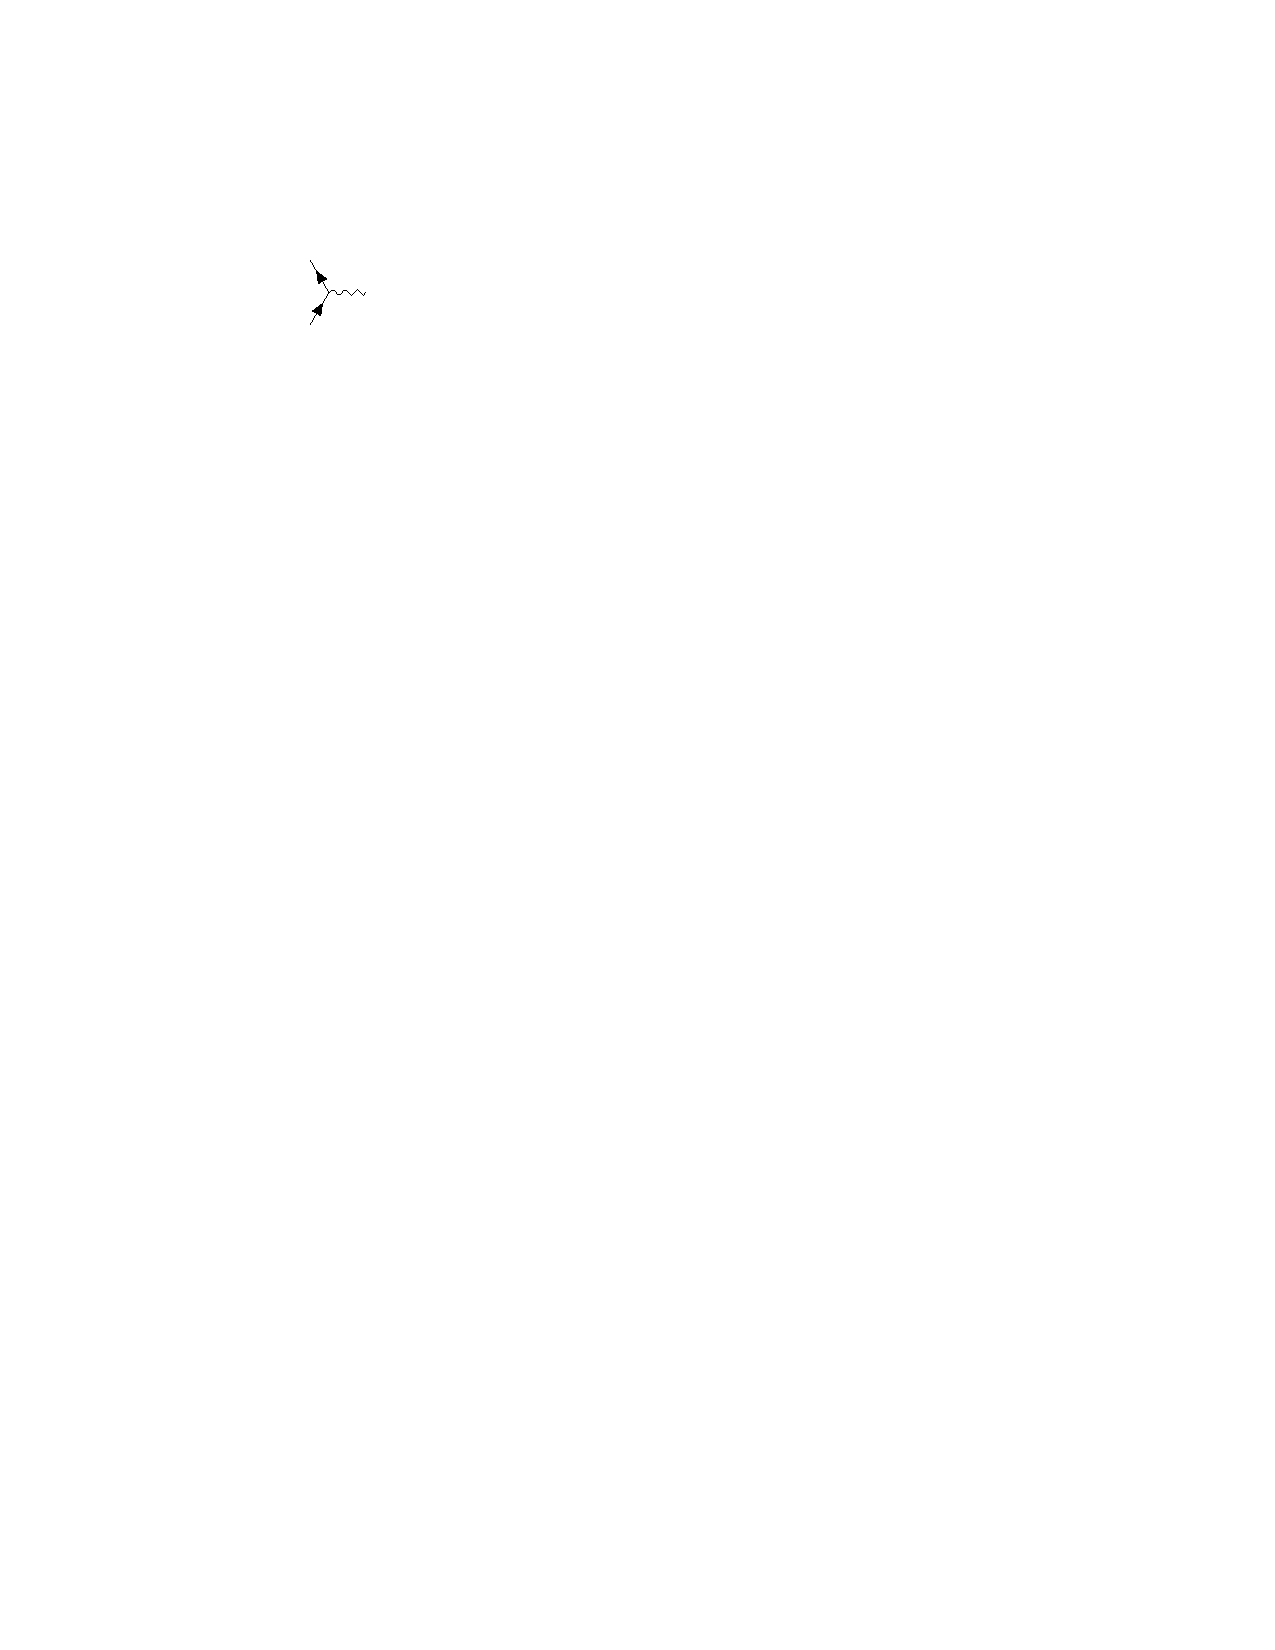
\includegraphics{Diagrams/eeg_vertex.pdf}}}={
i e_k \gamma^\mu
}
%\right]
%\qquad\text{respectively.}
\nonumber
}
where $\Gamma\ge0$ is a non-negative constant.
\begin{allparts}
\part
In a universe in which $0<m_1=m_2$, $0<\Gamma\ll m_1$ and $e_1 e_2>0$,  would it be possible for Bogus physicists looking at $e^+e^-\rightarrow \mu^+\mu^-$ data to determine that there are two types of Bogon rather than one?
Would anything change if we were to consider instead $e_1 e_2<0$ ? \marks{4}
\answer

The main point to make would be that any matrix element featuring one Bogon could be added to another having the other sort of Bogon substituted for it. Therefore every matrix element having an $\frac{e_1^2}{q^2-m^2+im\Gamma}$ (with the $e_1$ being squared as there will be a vertex factor at each end of the same Bogon) will end up added to another such that the resulting total matrix element would contain only terms of the form $\frac{e_1^2+e_2^2}{q^2-m^2+im\Gamma}$. Such a matrix element would be phenomenologically  indistinguishable from one derived from a theory in which there was only one bogon having single larger coupling constant $e$ satisfying $e^2=e_1^2+e_2^2$. Therefore there would be no way of deducing the existence of one rather than two Bogons.  Note that because of the presence of the squares of the coupling constants, signs are a red-herring here.
\endanswer
\end{allparts}
Suppose there are two Bogus universes $A$ and $B$, and that in each of these universes $0< m_1 < m_2$, $\Gamma=0$ and $e_1$ is equal to a non-zero constant $e$.  Further suppose that Universe $A$ has $e_2=0$ while Universe $B$ has $e_2=e$.  
\begin{allparts}
\part
For which range(s) of $\sqrt s$ (if any) is the tree-level cross section for the process $e^+ e^- \rightarrow \mu^+ \mu^-$ bigger in Universe $A$ than in Universe $B$, and for which range(s) of $\sqrt s$ (if any) is the reverse true?\marks{16}
\answer



The matrix element for $e^+e^-\rightarrow \mu^+\mu^-$ via two interfering massive bosons will be proportional to \alig{
j_e j_\mu \left(
\frac {e_1^2} {q^2-m_1^2+i m_1 \Gamma}
+
\frac {e_2^2} {q^2-m_2^2+i m_2 \Gamma}
\right)
}which is proportional to
\alig{e_1^2 z_1+e_2^2 z_2}where
\alig{
z_1&=
\frac 1 {q^2-m_1^2+i m_1 \Gamma}
%=
%\frac {q^2-m_1^2-i m_1 \Gamma } {(q^2-m_1^2)^2+ m_1^2 \Gamma^2}
%=
%\frac {q^2-M^2-i \epsilon M^2  } {(q^2-M^2)^2+ \epsilon^2M^4 %}
,\qquad\text{and}\\
z_2&=
\frac 1 {q^2-m_2^2+i m_2 \Gamma}
%=
%\frac {q^2-m_2^2-i m_2 \Gamma } {(q^2-m_2^2)^2+ m_2^2 \Gamma^2}
%=
%\frac {q^2-(2M)^2-i 2\epsilon M^2  } {(q^2-(2M)^2)^2+ 4\epsilon^2 M^4 }.
}
%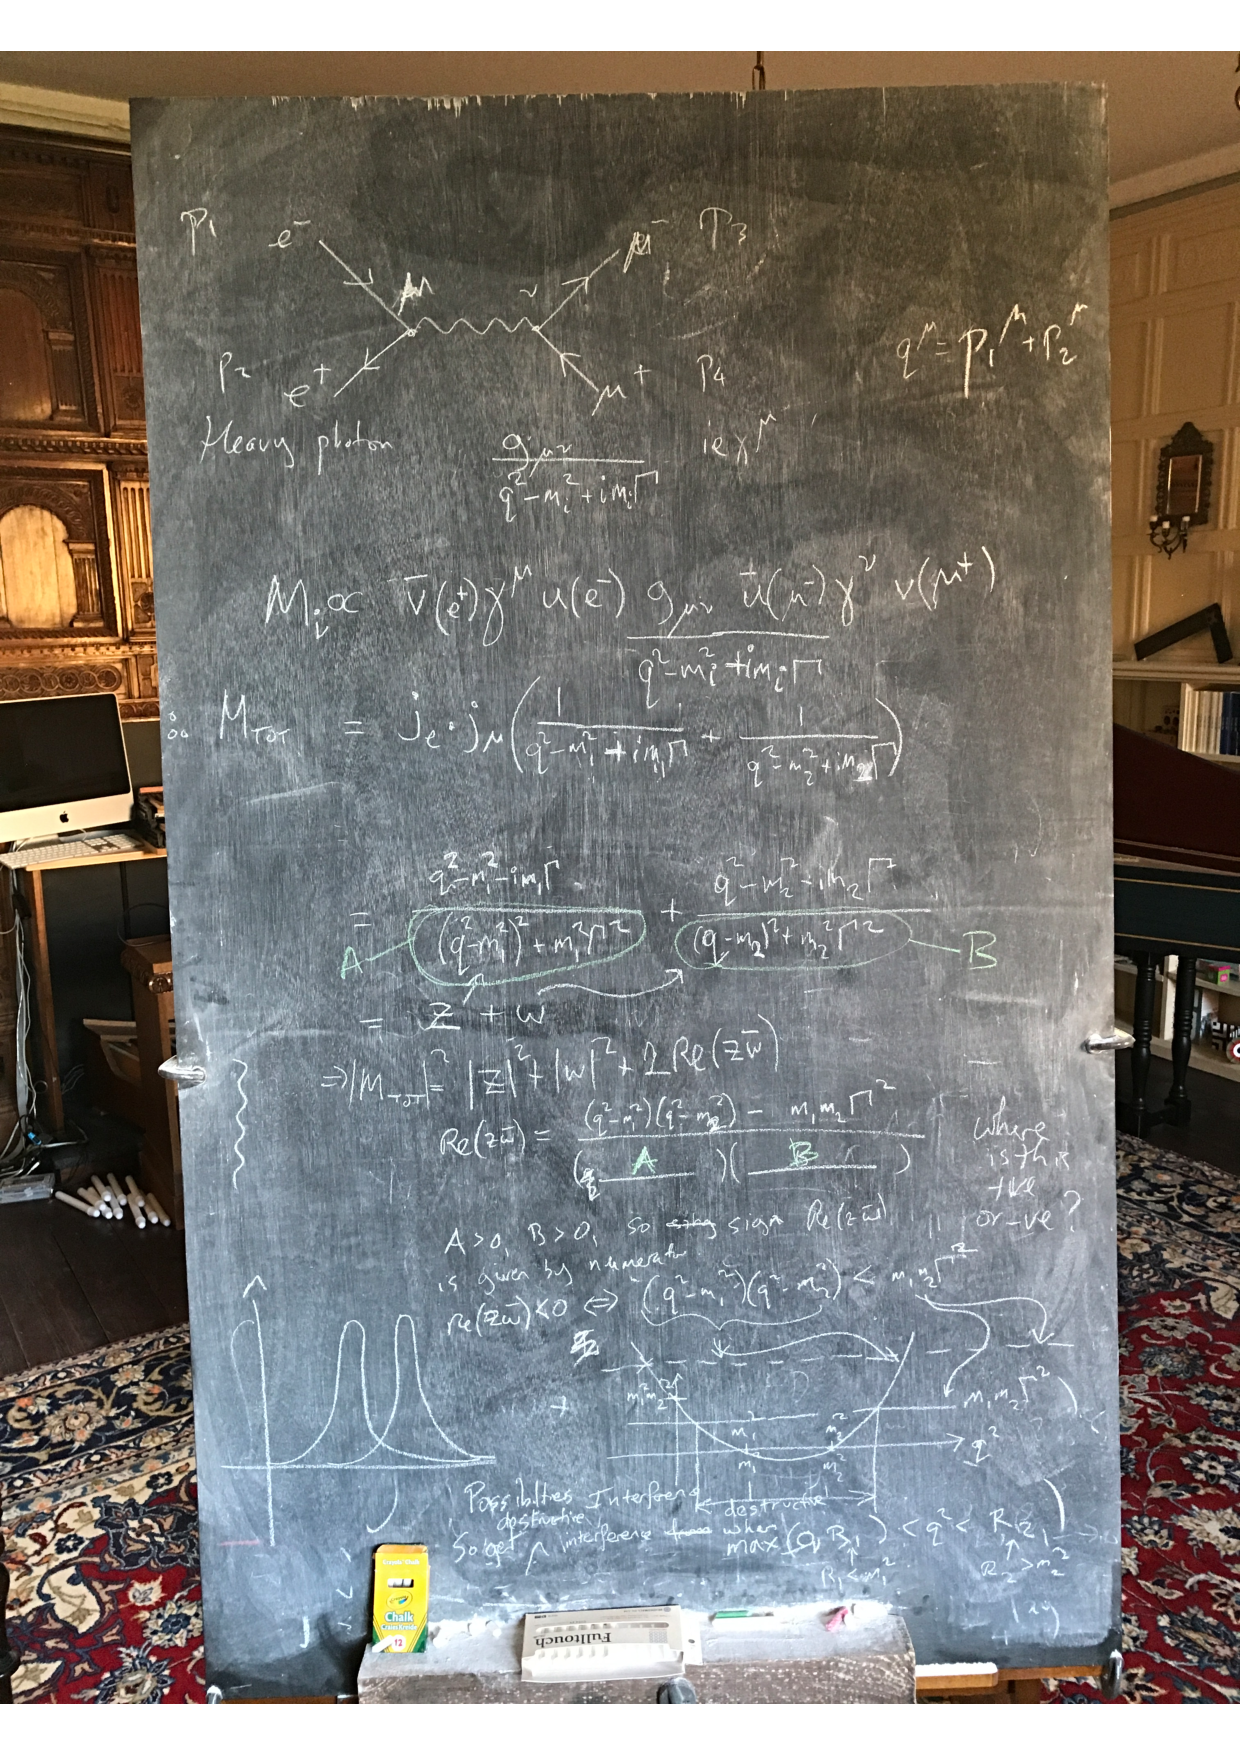
\includegraphics[height=15cm,width=15cm]{BogonMathsSketch}
%in either universe\alig{
%|M_{\text{tot}}|^2 
%&\propto
%|z_1+z_2|^2
%\\
%&=
%|z_1|^2
%+|z_2|^2
%+2 \Re\left[{z_1 z_2^*}\right]
%}and therefore
and hence\alig{
|M_{\text{tot}}|^2
&\propto |j_e\cdot j_\mu|^2\left|
e_1^2 z_1 + e_2^2 z_2
\right|^2
\\
&\propto\left|
e_1^2 z_1 + e_2^2 z_2
\right|^2.
}
If we consider the case which is mentioned in the question with  $\Gamma=0$, the complex numbers disappear from the question and we are left with
\alig{
|M_{\text{tot}}|^2
&\propto
\left(
e_1^2 z_1 + e_2^2 z_2
\right)^2
}
and hence, comparing the cross sections in the two universes\footnote{It is important to note that in this particular calculation only \textit{positive} constants has been dropped at each use of a proportional symbol ($\propto$).}:\alig{
\sigma_B-\sigma_A
&\propto
|M_{\text{tot(B)}}|^2
- 
|M_{\text{tot(A)}}|^2\nonumber
\\
&\propto
\left(
e^2 z_1 + e^2 z_2
\right)^2
-
\left(
e^2 z_1 + 0^2 z_2
\right)^2\nonumber
\\
&=
e^4\left(  (z_1+z_2)^2 - z_1^2\right)\nonumber
\\
&\propto
z_2^2+2 z_1 z_2\nonumber
\\
&=
z_2^2\left(1+\frac {2 z_1} {z_2}\right)\nonumber
\\
&=
1+\frac {2 z_1} {z_2}\label{eq:thingsketched}
}and hence\alig{
\left(\sigma_B >\sigma_A\right)
&\iff
\left( 1+\frac {2 z_1} {z_2} > 0\right)
\\
&\iff
\left(
1+\frac {2 (s-m_2^2)} {s-m_1^2} 
> 0\right).\label{eq:cond45}
}
The condition in \eqref{eq:cond45} is trivially true if both terms on the denominator have the same sign, which (given that $m_1^2<m_2^2$) happens if $\sqrt s<m_1$ or $\sqrt s>m_2$.  The only uncertainty relates to what happens when $s$ is in the intermediate position: $m_1^2 \le s \le m_2^2$. In this intermediate zone we have:
\alig{
\left(
1+\frac {2 (s-m_2^2)} {s-m_1^2} 
> 0\right)
&\iff
\left(
(s-m_1^2)+2 (s-m_2^2)  
> 0\right)
\\
&\iff
\left(
3s  
> m_1^2+2m_2^2
\right)
\\
&\iff
\left(
\sqrt s  > \sqrt{\frac 1 3 \left(m_1^2+2m_2^2\right)
}\right)
}therefore, considering all non-negative $\sqrt s$ we see that
\alig{
\left(\sigma_B \le \sigma_A\right)
&\iff
\left[
m_1\le\sqrt s\le\sqrt{\frac 1 3 \left(m_1^2+2m_2^2\right)}
\right]
}which is perhaps best summarized in the following sketches (in which the quantity on the RHS of  \eqref{eq:thingsketched} is called $f(\rho(\sqrt s))$):
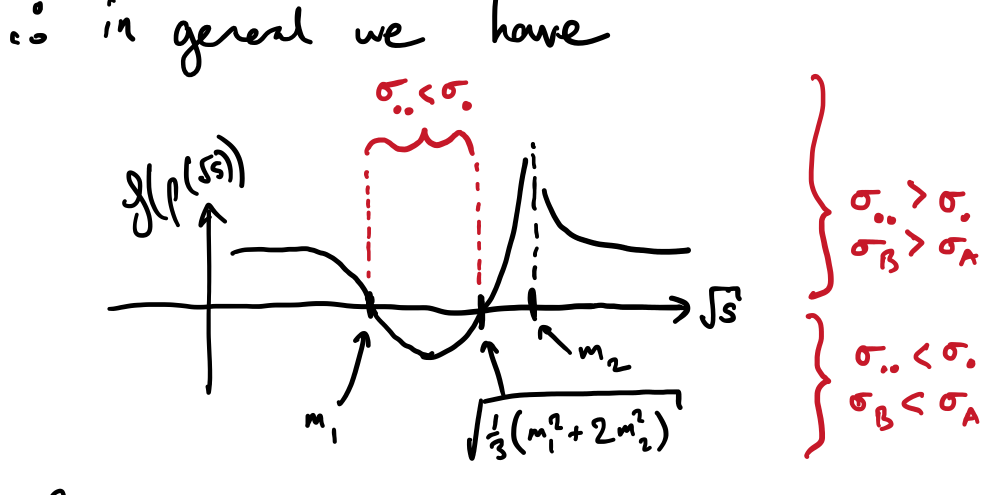
\includegraphics[width=\textwidth]{cropped_working_diag}



\hide{Hence, comparing the two universes:\alig{
|M_{\text{tot(B)}}|^2
- 
|M_{\text{tot(A)}}|^2
&\propto
\left(
e^4|z_{1}|^2
+e^4|z_{2}|^2
+2 e^2 e^2\Re\left[{z_{1}^* z_{2}}\right]
\right)\nonumber
-\left(
e^4|z_{1}|^2
+0^4|z_{2}|^2
+2e^2 0^2 \Re\left[{z_{1}^* z_{2}}\right]
\right)
\\
&\propto
\left(
|z_{1}|^2
+|z_{2}|^2
+2 \Re\left[{z_{1}^*z_{2}}\right]
\right)
-
|z_{1}|^2
\nonumber
\\
&=
|z_{2}|^2
+2 \Re\left[{z_{1}^* z_{2}}\right]
\nonumber
\\
&=
|z_{2}|^2
+2 |z_{1}||z_{2}|\cos\left({\arg {z_2}-\arg{z_1}}\right)
\nonumber
\\
&\propto
\frac {|z_{2}|}{|z_{1}|}
+2 \cos\left({\arg {z_2}-\arg{z_1}}\right)
\nonumber
%\\
%&=
%\frac {|z_{2}|}{|z_{1}|}
%+2 \cos\left({\arg {z_2}-\arg{z_1}}\right)
%\nonumber
\\
&=
\left|\frac {z_{2}}{z_{1}}\right|
+2 \cos\left({\arg \frac{z_2} {z_1}}\right)
\nonumber
\\
&=|\rho| + 2\cos\arg\rho
\\
&\underset{\text{def}}{\equiv} f(\rho)
%&=
%\left| \frac {|1/z_{1}|}{|1|/z_{2}} \right|
%2 \cos\left({\arg {\frac 1 {z_2}}-\arg{\frac 1 {z_1}}}\right)
%\nonumber
%\\
%&=
%\frac {|(s-m_1^2) + i m_1 \Gamma|}{|(s-m_2^2) + i m_2 \Gamma|}
%+2 \cos\left({\arctan {\frac {m_2 \Gamma} {s-m_2^2}}-\arctan{\frac {m_1 \Gamma} %{s-m_1^2}}}\right)
%\nonumber
}where\alig{
\rho &= \frac {z_2}{z_1} = \frac {(s-m_1^2) + i m_1 \Gamma}{(s-m_2^2) + i m_2 \Gamma}.
}
The evaluation of where $f(\rho)$ is posisitive or negative then continues as follows:
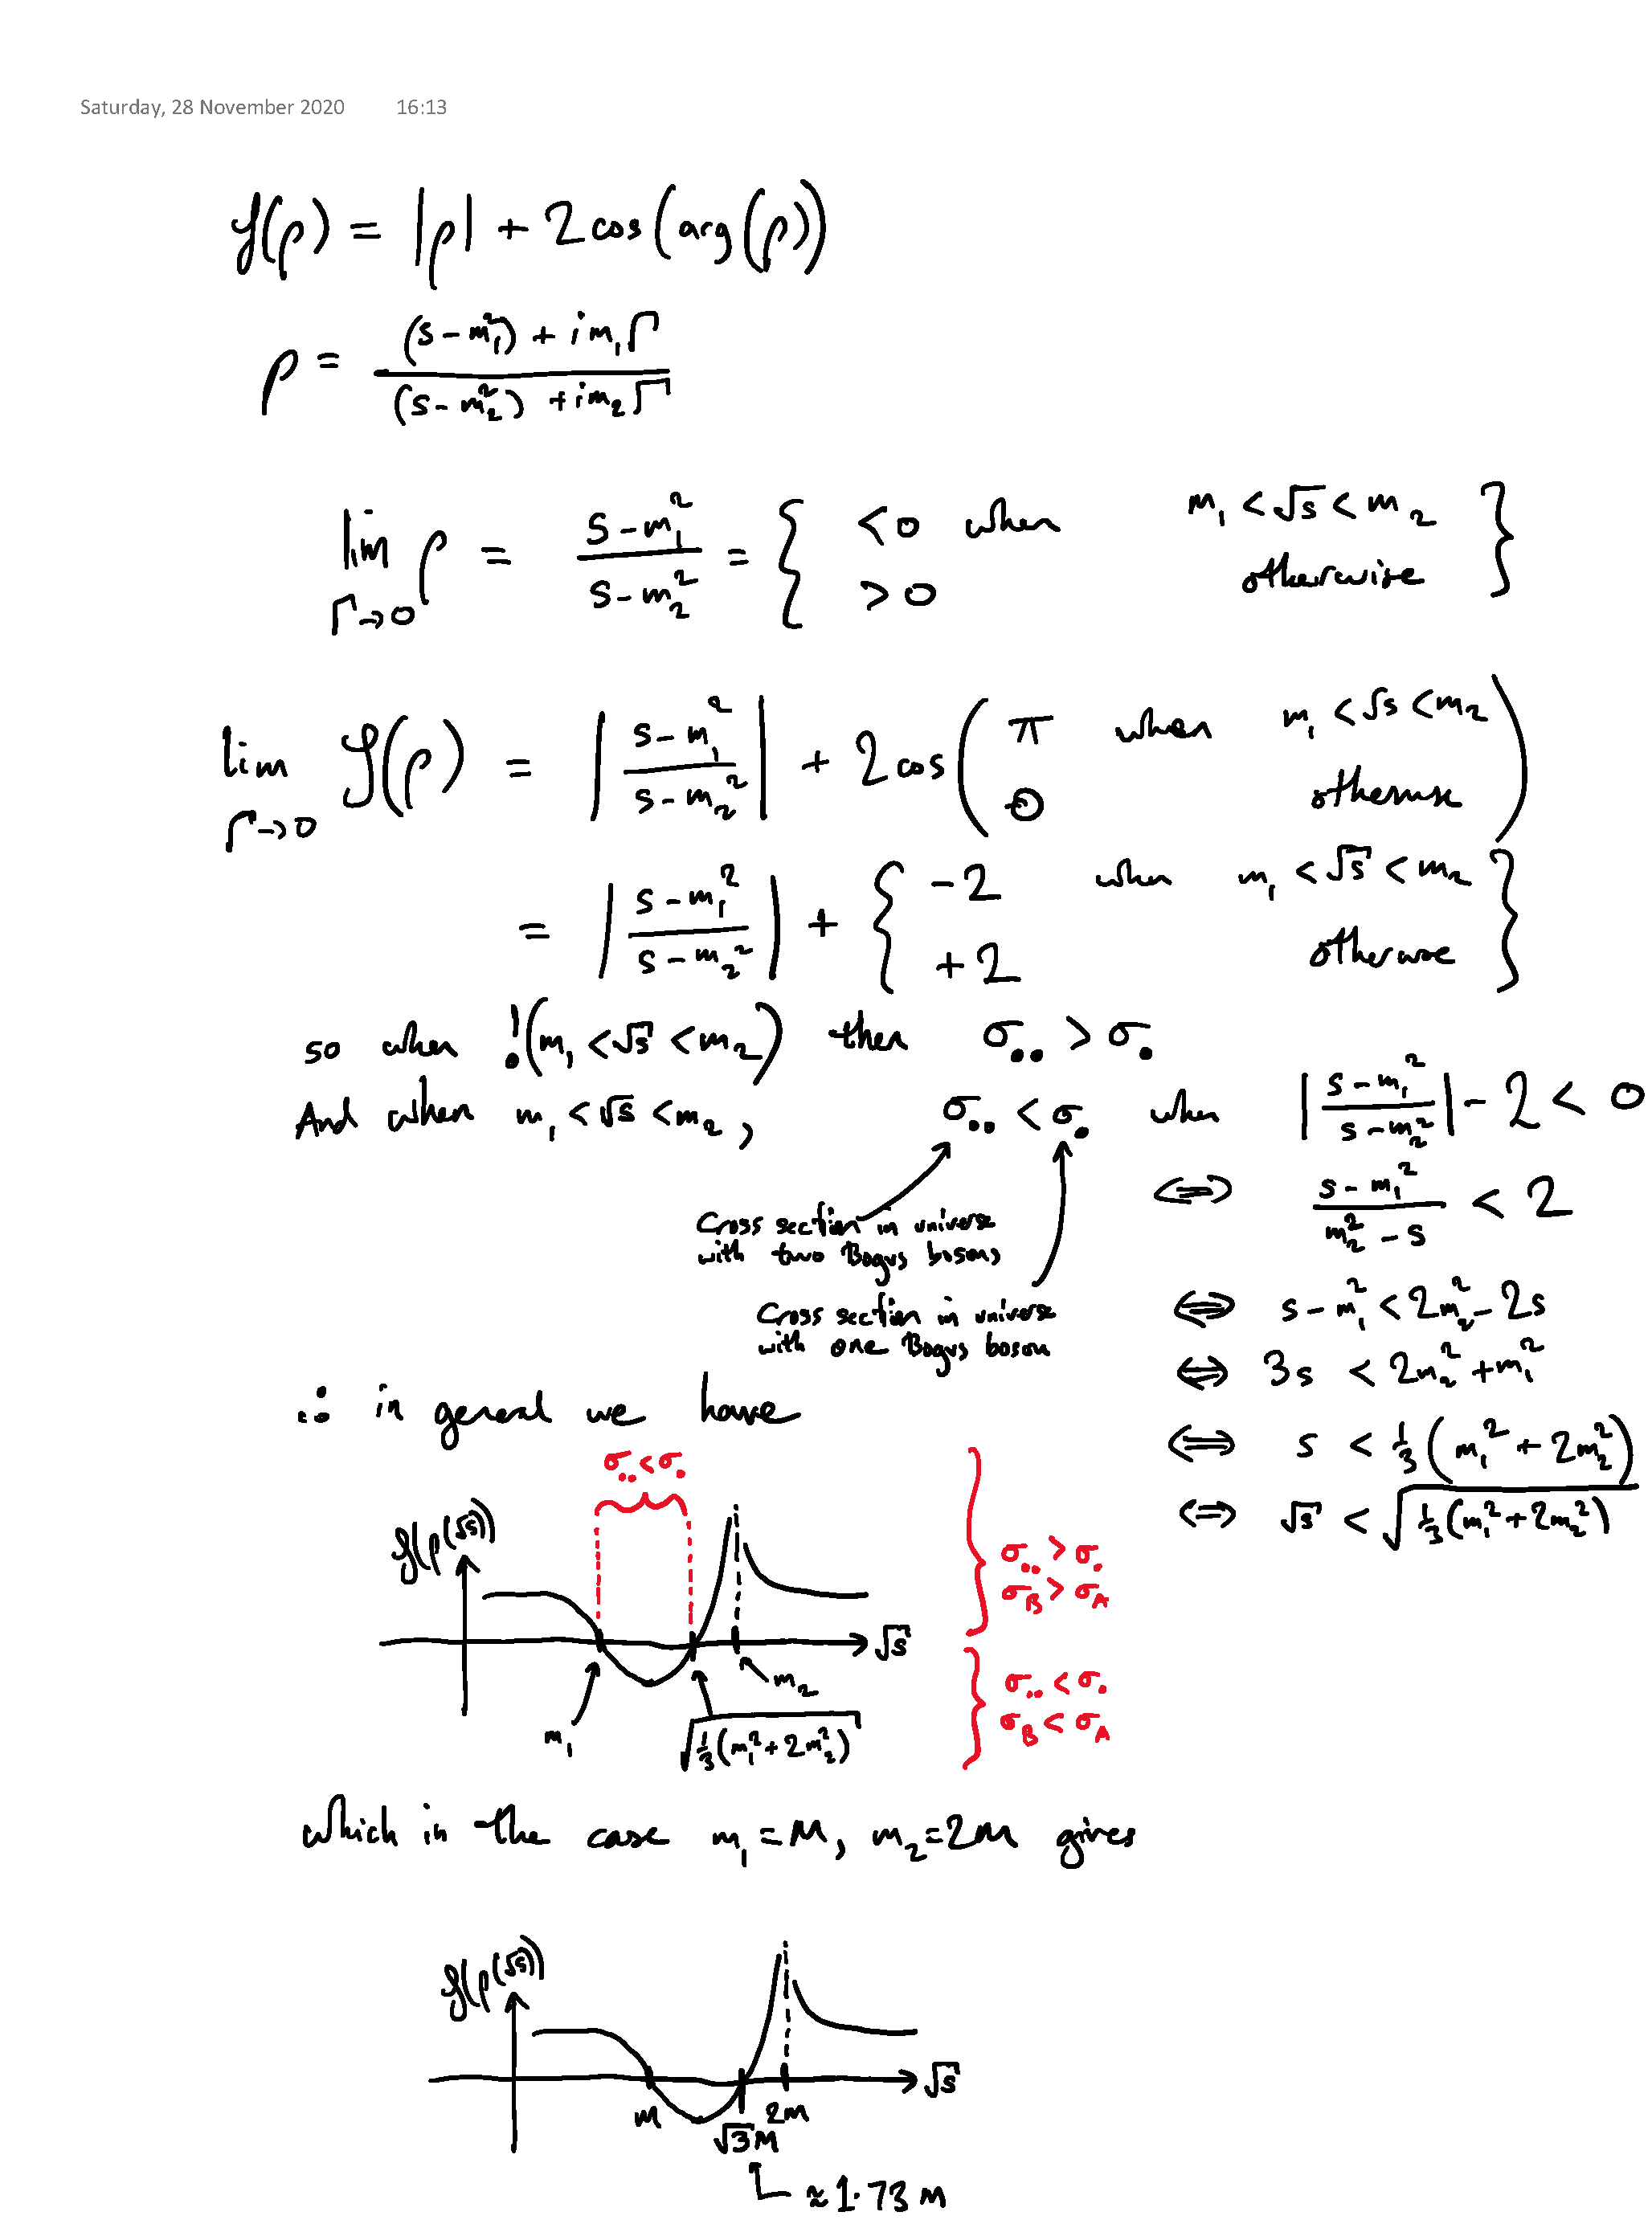
\includegraphics[width=0.9\textwidth]{working}


So the cross section for our process in  universe B is less than in universe A when (and only when) $f(\rho)<0$.  What do we need for this to happen?   Since $|\cos\rho|\le 1$ for all $\rho$, it is clearly an absolute requirement that $\rho$ itself is less than two.  Or put another way:\alig{(|\rho|\ge2) &\implies (f(\rho)\ge0).}   
}
\endanswer
\end{allparts}
A `Bogus $e^+e^-$ Collider' previously only able to reach centre of mass energies of up to $\sqrt s=9m_2$ is upgraded to allow it also to access the region $9m_2<\sqrt s<10 m_2$.  A team of Bogus physicists (who believe themselves to live in Universe B) find that  the $e^+e^-\rightarrow \mu^+\mu^-$ cross section measured by the collider in the new energy region appears    to undershoot the theoretical predictions made by their (previously reliable) Bogus Standard Model.
\begin{allparts}
\part
What conclusion(s) might these physicists draw from the new data? \marks{3}
\answer

In the last part of the question we have seen that between two narrow-width bosons there will inevitably be a region in which interference from the heavier boson makes the total cross section lower than you'd otherwise expect, strange though this seems.  Therefore, the physicists, after first concluding that their standard model was wrong, might tentatively hazard a guess that a new boson was about to appear with a mass somewhere beyond $10m_2$.
\endanswer
\end{allparts}
A %fictional economic meltdown brought about by a fictional government's responses to a fictional plot-device which overly-risk averse external examiners have not permitted me to name on this paper precipitates an imaginary 
funding crisis in physics %which
prohibits the construction of further energy upgrades to the Bogus $e^+e^-$ Collider. 
\begin{allparts}
\part
 What  would you recommend the aforementioned physicists should do to get the most out of the machine they already have? \marks{3}
 \answer
 
 This is a fairly open-ended question, so any sensible thoughtful  answer here will get credit, even if it is not on precisely the same train of thought as the examiner.   Nonetheless, what the examiner has in mind is that candidates will note from the previous answer that there is evidence that there is evidence that there is a new `third' boson just beyond the range of the current collider. Consequently, although they may not be able to make that boson directly, they could perhaps get an indirect measurement of its mass by looking very precisely  deviation of the cross section from their naive two-boson model.  In principle, the shape and size of the deviation completely encapsulates the rest of the spectrum, though in practice the deviations are very small and the extrapolation will have large uncertainties.  In particular, a very heavy boson with a stronger coupling might have similar foothills to a lighter boson with a weaker coupling.  Consequently the uncertainties on the indirect measurements of the coupling and mass of the third boson are likely to be correlated.
 
 It would be interesting to see if any students suggest trying to polarise the beams. [The question notes that \textbf{energy} upgrades are impossible, but doesn't explicitly rule out other forms of upgrade.]
 \endanswer
\end{allparts}

\clearpage

\question 

The second handout of this year's lecture course derived many properties of spinors and the Dirac equation assuming the usual `$3D$' Minkowski spacetime having one time and three space dimensions.  
Which of those properties would remain the same, and which would change (and how) assuming instead a `$2D$' spacetime having two space dimensions in addition to time?  \marks{30}

\vspace{5mm}

Credit will be given for the quality of the arguments which relate specifically to the $2D$ case, and the degree to which they convey to the marker the sense that the candidate understands the physics and concepts underlying the Dirac equation, spinors and fermions.  No credit will be given for merely reporting what happens in $3D$, though comparisons between $2D$ and $3D$ are encouraged if they help to explain important features of the $2D$ spinors.

\vspace{5mm}

Candidates may wish to structure an answer around some of the following questions, though no candidate is required to give answers to all of them, and no candidate is forbidden from discussing other questions which they feel are relevant:
\begin{enumerate}
\item\ 
What are the number, dimensions and required commutation or anticommutation relations of the smallest  $\alpha$ and $\beta$ matrices that a $2D$ Dirac Hamiltonian should use?
\item\ 
Does it remain sensible to create $\gamma$ matrices from $\alpha$ and $\beta$ matrices, and if so in what way?
\item\ 
Does the Dirac equation take a new form in $2D$~?
\item\ 
Does it remain beneficial to create $v$-spinors in addition to $u$-spinors?
\item\ 
Does the $2D$ theory predict both particles and anti-particles?
\item\ 
Do states still carry intrinsic spin angular momentum?
\item\ 
What explicit form (or forms) might a $2D$ spinor  take for a particle of mass $m$ having energy $E$ and momentum $(p_x,p_y)$ within the spatial two-space?   
\item\ 
Certain $3D$-spinor wave functions change sign when subjected to $2\pi$ rotations about certain axes. Is there anything analogous  for spinors in $2D$~? 
\end{enumerate}



\answer

%Will the students find \url{http://www.rhysdavies.info/physics_page/resources/notes/spinors.pdf} after googling `spinors in two dimensions' as I did?
The Dirac Hamiltonian would still start of being formulated as\alig{
H = \vec \alpha\cdot\vec p + \beta m }giving\alig{
H^2 
&= (\vec \alpha\cdot\vec p + \beta m)(\vec \alpha\cdot\vec p + \beta m)
\\
&= 
\alpha_x \alpha_x p_x^2
+\alpha_y \alpha_y p_y^2
+\beta^2 m^2\\
&\qquad
+p_x p_y \left(
\alpha_x \alpha_y
+
\alpha_y \alpha_x 
\right)
+m p_x (\beta \alpha_x + \alpha_x \beta) 
+m p_y (\beta \alpha_y + \alpha_y \beta) 
}yet we desire:
\alig{
H^2=p_x^2+p_y^2+m^2
}so need
\alig{
\anticom {\alpha_x} {\alpha_y} = \anticom {\alpha_x} {\beta} = \anticom {\alpha_y} {\beta} &= 0\\
\anticom {\alpha_x} {\alpha_x} = \anticom {\alpha_y} {\alpha_y} = \anticom {\beta} {\beta} &= 2 
}Can't do above with real or complex numbers since we evidently need non-zero quantities which can anticommute with each other.
But we can use 2x2 matrices, indeed the usual Pauli matrices $\sigma_1$, $\sigma_2$ and $\sigma_3$ would suffice since they each square to $\unit_{2\times 2}$ as well as satisfying
\alig{
\sigma_1 \sigma_2 &= +i \sigma_3\qquad\text{(and cyclic perms)},
\\
\sigma_2 \sigma_1 &= -i \sigma_3\qquad\text{(and cyclic perms),}
}
and so (for example)
\alig{
\anticom{\sigma_1}{\sigma_2}
&=
\sigma_1 \sigma_2 + \sigma_2 \sigma_1
\\
&=
i \sigma_3 -i \sigma_3
\\
&=0.
}
Mostly we can avoid using any specific representation ... but for those cases where a particular representation is unavoidable it may be sensible to use:
\alig{
\alpha_x=\sigma_1&=
\matTwoTwo
0 1 1 0
,\\
\alpha_y=\sigma_2&=
\matTwoTwo
0  {-i} i  0,\\
\beta=\sigma_3&=
\matTwoTwo
1  0 0  {-1}
}in which $\beta$ is chosen to be diagonal to match the Pauli-Dirac convention we used in lectures.

If we did use the above representation, then our Dirac Hamiltonian would take the form
\alig{
H &= \matTwoTwo 
{m} {p_x-i p_y} 
{p_x+i p_y} {-m}.
}
Defining
\alig{
\gamma^0 &= \beta,\\
\gamma^1 &= \beta \alpha_x,\\
\gamma^2 &= \beta \alpha_y
}%
we note that 
\alig{
\hat H \psi &= i \partial_t \psi
}%
implies
\alig{
0 
&= i \partial_t \psi - \hat H \psi
\\
&= \left(i \partial_t  - \vec \alpha \cdot \vec {\hat  p} - \beta m \right)\psi
\\
&= \left(i \partial_t  + i \vec \alpha \cdot \vec \partial - \beta m \right)\psi
\\
&= \beta \left(i \partial_t  + i \vec \alpha \cdot \vec \partial - \beta m \right)\psi
\\
&=  \left(i \gamma^0\partial_t  + i \vec \gamma \cdot \vec \partial - \beta^2 m \right)\psi
\\
&=  \left(i \gamma^\mu\partial_\mu - m \right)\psi
}%
in just the same way as in $1+3$ space time dimensions.  In other words, the Dirac equation doesn't look any different notationally, even though it contains one fewer gamma matrix.

[BEGIN ASIDE:

In our rep
\alig{
\gamma^0 &= \sigma_3 = \matTwoTwo 1 0 0  {-1}=(\gamma^0)^*,\label{eq:conjourgam0}\\
\gamma^1 &= \sigma_3 \sigma_1 = i \sigma_2 = \matTwoTwo 0 1
{-1} 0 = (\gamma^1)^*,\label{eq:conjourgam1}\\
\gamma^2 &= \sigma_3 \sigma_2 = i \sigma_1 = \matTwoTwo 0 i i 0 = -(\gamma^2)^*.\label{eq:conjourgam2}
}%

END ASIDE]

For plane wave solutions:
\alig{
\psi_u = u e^{-i p_\mu x^\mu}\qquad\text{and}\qquad\psi_v = v e^{+i p_\mu x^\mu}
}%
we have therefore
\alig{
\left(i \gamma^\mu (-i)p_\mu - m \right)u &= 0, \qquad\text{and}\\
\left(i \gamma^\mu (+i)p_\mu - m \right)v &= 0
}%
i.e.~
\alig{
\left(\gamma^\mu p_\mu - m \right)u &= 0,\qquad\text{and}\\
\left(\gamma^\mu p_\mu + m \right)v &= 0
}%
which are likewise unchanged from the usual forms.
Going slightly back on ourselves:
\alig{
\beta\left(\gamma^\mu p_\mu - m \right)u &= 0,\qquad\text{and}\\
\beta\left(\gamma^\mu p_\mu + m \right)v &= 0
}%
implies
\alig{
\left(
 E 
-\alpha_x p_x 
-\alpha_y p_y  
- \beta m \right)u &= 0,\qquad\text{and}\\
\left(
 E 
-\alpha_x p_x 
-\alpha_y p_y  
+ \beta m \right)v &= 0.
}%
which can be written as 
\alig{
(E-H_{\vec p})u&=0,\qquad\text{and}\label{eq:eu}\\
(E+H_{-\vec p})v&=0\label{eq:ev}
}%
in which the subscripts indicate whether to use the `normal' $\vec p$ or its negated version in the Hamiltonian.
Considering just the $u$ version of the two equations above:
\alig{
0&=(H_{\vec p}-E)u
\\
&= \matTwoTwo 
{-E+m} {p_x-i p_y} 
{p_x+i p_y} {-E-m} 
\vecTwo {u_1}{u_2}
}%
and so
\alig{
(-E+m) u_1 + (p_x-i p_y) u_2 = 0\label{eq:worstuform}
}%
and so
\alig{
u \propto \vecTwo {p_x - i p_y} {E-m}.
}%
Alternatively, we could have written
\alig{
(p_x+i p_y)u_1-(E+m)u_2=0
}%
which would have lead to
\alig{
u &\propto \vecTwo {E+m} {p_x+i p_y}.\label{eq:bestuform}
}%

Note: The above two kinds of $u$ are equivalent since 
\alig{
\frac{E+m}{p_x-i p_y}\vecTwo {p_x - i p_y} {E-m}
&=
\vecTwo {E+m} {\frac{(E+m)(E-m)}{p_x-i p_y}}
\\
&=
\vecTwo {E+m} {\frac{(E^2-m^2)(p_x+i p_y)}{(p_x-i p_y)(p_x+i p_y)}}
\\
&=
\vecTwo {E+m} {\frac{(E^2-m^2)(p_x+i p_y)}{p_x^2+p_y^2}}
\\
&=
\vecTwo {E+m} {\frac{(E^2-m^2)(p_x+i p_y)}{E^2-m^2}}
\\
&=
\vecTwo {E+m} {p_x+i p_y}.
}

Given that they are equivalent, it may be better to use the form shown in \eqref{eq:bestuform} since it is in a form where one can take momenta to zero easily (i.e.~without neading to use L'Hopital's rule). 

Putting in a normalisation factor
\alig{
u = k_u \vecTwo {E+m}{p_x + i p_y} 
}%
and requiring that $u^\dag u=2 E$ we can see that
\alig{
2E 
&= 
|k_u^2|  \vecTwo{E+m}{p_x + i p_y}  ^\dag \vecTwo{E+m}{p_x + i p_y} 
\\
&=
|k_u^2|  \left((E+m)^2+p_x^2+p_y^2\right)
\\
&=
|k_u^2|  \left(E^2+2 E m+m^2+p_x^2+p_y^2\right)
\\
&=
|k_u^2|  \left(2 E m+2E^2\right)
\\
&=
2E |k_u^2|  \left(E+m\right)
}%
and hence
\alig{
k_u
&=
\frac{1}{\sqrt{E+m}}
}%
and so our normalised $u$-spinor takes the form
\alig{
u &= \frac{1}{\sqrt{E+m}} 
\vecTwo {E+m}{p_x+ip_y}\label{eq:bestnormaizeduform}
}%
which is much nicer than following alternative which (though correct) is much more difficult to work with for particles moving slowly:
\alig{
u &= \frac 1 {\sqrt{E-m}} \vecTwo {p_x - i p_y} {E-m}.
}(The second form would have resulted from using \eqref{eq:worstuform} instead of \eqref{eq:bestuform} as the starting point for the normalisation.)


We can also check that our $u$-spinors have the eigenvalue expected from \eqref{eq:eu}.
\alig{
H_{\vec p} \ u &=
\frac 1 {\sqrt{E-m}}\matTwoTwo 
{m} {p_x-i p_y} 
{p_x+i p_y} {-m}
\vecTwo {p_x - i p_y} {E-m}
\\
&=
\frac 1 {\sqrt{E-m}}\vecTwo
{(p_x - i p_y)(m+(E-m))}
{p_x^2+p_y^2+m^2-E m}
\\
&=
\frac 1 {\sqrt{E-m}}\vecTwo
{(p_x - i p_y)(+E)}
{E^2-E m}
\\
&=E
\frac 1 {\sqrt{E-m}}\vecTwo
{p_x - i p_y}
{E- m}
\\
&=E u
\qquad\text{(Q.E.D.)}.
}
By comparing \eqref{eq:eu} and 
\eqref{eq:ev} we can see that the $v$ solutions will be obtainable from the $u$ solutions by substituting $-E$ for $E$ and $-\vec p$ for $\vec p$ and hence
\alig{
v \propto \vecTwo {-p_x + i p_y} {-E-m} \propto \vecTwo {p_x - i p_y} {E+m}
}
or in normalised form:
\alig{
v = \frac{1}{\sqrt{E+m}}\vecTwo {p_x - i p_y} {E+m}.\label{eq:bestnormaizedvform}
}
For this solution:
\alig{
H_{\vec p} \ v &\propto
%\frac 1 {\sqrt{E+m}}
\matTwoTwo 
{m} {p_x-i p_y} 
{p_x+i p_y} {-m}
\vecTwo {p_x - i p_y} {E+m}.\\
&=
%\frac 1 {\sqrt{E+m}}
\vecTwo
{(p_x - i p_y)(m+(E+m))}
{p_x^2+p_y^2-Em - m^2}
\\
&=
%\frac 1 {\sqrt{E+m}}
\vecTwo
{(p_x - i p_y)(E+2m))}
{(p_x^2+p_y^2+m^2)-Em -2 m^2}
\\
&=
%\frac 1 {\sqrt{E+m}}
\vecTwo
{(p_x - i p_y)(E+2m)}
{E^2-Em-2m^2}
\\
&=
\vecTwo
%\frac 1 {\sqrt{E+m}}
{(p_x - i p_y)(E+2m)}
{E^2-m(E+2m)}
}
YUK!!!  For reasons seen below, should use $H_{-\vec p}$ instead.

Here is reason:
\alig{
\hat H - i \partial_t
&=
\vec \alpha\cdot  \vec{\hat p} + \beta m- i \partial_t
\\
&=
\vec \alpha\cdot  (-i\vec\partial)+ \beta m- i \partial_t
\\
&=
\matTwoTwo
{+m-i\partial_t}   {(-i\partial_x)-i(-i\partial_y)}
{(-i\partial_x)+i(-i\partial_y)}     {-m-i\partial_t}
\\
&=
\matTwoTwo
{+m-i\partial_t}   {-i\partial_x-\partial_y}
{-i\partial_x+\partial_y}     {-m-i\partial_t}
}%
so
\alig{
 i \partial_t-\hat H 
&=
\matTwoTwo
{-m+i\partial_t}   {i\partial_x+\partial_y}
{i\partial_x-\partial_y}     {m+i\partial_t}
}%
and so
\alig{
( i \partial_t-\hat H ) 
\psi_u 
&=
( i \partial_t-\hat H )
u e^{-i p_\mu x^\mu}
\\
&\propto
\matTwoTwo
{-m+i\partial_t}   {i\partial_x+\partial_y}
{i\partial_x-\partial_y}     {m+i\partial_t}
\vecTwo {p_x - i p_y} {E-m}
e^{-iE t + i\vec p \cdot \vec x}
\\
&=
\matTwoTwo
{-m+i(-iE)}   {i(i p_x)+(i p_y)}
{i(i p_x)-(i p_y)}     {m+i(-i E)}
\vecTwo {p_x - i p_y} {E-m}
e^{-iE t + i\vec p \cdot \vec x}
\\
&=
\matTwoTwo
{-m+E}   {- p_x+i p_y}
{-p_x-i p_y}     {m+ E}
\vecTwo {p_x - i p_y} {E-m}
e^{-iE t + i\vec p \cdot \vec x}
\\
&=
\vecTwo
{(p_x-i p_y)((-m+E)+(-E+m)}
{-p_x^2-p_y^2-m^2+E^2}
e^{-iE t + i\vec p \cdot \vec x}
\\
&=
\vecTwo 0 0
}%
while
\alig{
( i \partial_t-\hat H ) 
\psi_v 
&=
( i \partial_t-\hat H )
v e^{+i p_\mu x^\mu}
\\
&\propto
\matTwoTwo
{-m+i\partial_t}   {i\partial_x+\partial_y}
{i\partial_x-\partial_y}     {m+i\partial_t}
\vecTwo {p_x - i p_y} {E+m}
e^{iE t - i\vec p \cdot \vec x}
\\
&=
\matTwoTwo
{-m+i(iE)}   {i(-ip_x)+(-ip_y)}
{i(-ip_x)-(-ip_y)}     {m+i(iE)}
\vecTwo {p_x - i p_y} {E+m}
e^{iE t - i\vec p \cdot \vec x}
\\
&=
\matTwoTwo
{-m-E}   {p_x-ip_y}
{p_x+ip_y}     {m-E}
\vecTwo {p_x - i p_y} {E+m}
e^{iE t - i\vec p \cdot \vec x}
\\
&=
\vecTwo
{(p_x-ip_y)((-m-E)+(E+m))}
{p_x^2+p_y^2+m^2-E^2}
e^{iE t - i\vec p \cdot \vec x}
\\
&=
\vecTwo 0 0
}%
and so both $\psi_u$ and $\psi_v$ are valid solutions.  In showing that the above solutions work, we have not made use of any requirements that $E$ be positive, and indeed in all cases the proofs only require that $E^2=p_x^2+p_y^2+m^2$ and so work for any real $E$.  Presumably we could therefore use just the $u$ spinors, but remember to have both positive and negative $E$, or alternatively we could use only positive $E$ everywhere but use both $u$ and $v$ spinors.

\subsubsection{Charge conjugation?} 

Our Dirac equation was
\alig{
0
&=  \left(i \gamma^\mu\partial_\mu - m \right)\psi
}just as in $SO(3,1)$.  Lectures noted that if we replace
\alig{\partial_\mu \rightarrow \partial_\mu + i e A_\mu}%
then we can attempt to see what manipulations lead to charge conjugation of a spinor.  In lectures for $SO(3,1)$ we found that the charge conjugation operator was
\alig{
C : \psi \rightarrow \psi' = C \psi = i \gamma^2 \psi^*.\label{eq:chargeconjugationoperator}
}%
The argument used in lectures used $\gamma^2$ rather than some other gamma matrix because of the following special property of $\gamma^2$ which held in the particular representation which the lectures used:
\alig{
(\gamma^0)^* &= (\gamma^0)
\\
(\gamma^1)^* &= (\gamma^1)
\\
(\gamma^2)^* &= - (\gamma^2)
\\
(\gamma^3)^* &= (\gamma^3), \qquad\text{and}
\\
\gamma^2 (\gamma^\mu)^* &= -\gamma^\mu \gamma^2.\label{eq:sduhjhbdsd}
}%
The same argument will work again here if our three gammas satisfy the above relations too (ignoring the unnecessary $\gamma^3$). We can already see from \eqref{eq:conjourgam0},\eqref{eq:conjourgam1} and \eqref{eq:conjourgam2}  that the first three conditions above are satisfied in our rep.  The last constraint \eqref{eq:sduhjhbdsd} then follows from the first three together with the fact that dissimilar gamma matrices anticommute.
We therefore conclude that even in $SO(3,1)$ the charge conjugation operator remains (for our choice of representation) exactly as shown in \eqref{eq:chargeconjugationoperator}.

We therefore investigate:
\alig{
C \psi_u &= 
i \gamma^2 \psi_u^*  
\\
&\propto 
i \matTwoTwo 0 i i 0  \left(\vecTwo {p_x-i p_y} {E-m} e^{ -i p_\mu x^\mu}\right)^*  
\\
&= 
\matTwoTwo 0 {-1} {-1} 0  \vecTwo {p_x+i p_y} {E-m} e^{ +i p_\mu x^\mu} 
\\
&= 
  -\vecTwo {E-m}  {p_x+i p_y} e^{ +i p_\mu x^\mu} 
\\
&\propto
  \frac{p_x -i p_y}{E-m}
  \vecTwo {E-m}  {p_x+i p_y} e^{ +i p_\mu x^\mu} 
\\
&=
  \vecTwo {p_x -i p_y}  {\frac{(p_x -i p_y)(p_x+i p_y)} {E-m} } e^{ +i p_\mu x^\mu} 
\\
&=
  \vecTwo {p_x -i p_y}  {\frac{
  p_x^2+p_y^2
  } {E-m} } e^{ +i p_\mu x^\mu} 
\\
&=
  \vecTwo {p_x -i p_y}  {\frac{
  E^2-m^2
  } {E-m} } e^{ +i p_\mu x^\mu} 
\\
&=
  \vecTwo {p_x -i p_y}  {\frac{
 (E-m)(E+m)
  } {E-m} } e^{ +i p_\mu x^\mu} 
\\
&=
  \vecTwo {p_x -i p_y}  {E+m} e^{ +i p_\mu x^\mu} 
\\
&\propto
  \psi_v
}%
which shows us that the $u$ spinors are antiparticles of the $v$ spinors, and vice versa.

\subsubsection{Angular momentum}
In $SO(2,1)$ things cannot rotate about axes in the plane, but they can rotate about a vertical axis (i.e.~an in-plane rotation). Noting that we really want an analogue of the `angular-momentum-about-the-$z$-axis' operator of $SO(2,1)$ (i.e.~$(\vec{\hat r} \times \vec {\hat p})_z$) we might call our in-plane angular momentum operator $\hat L$ and define it as follows: \alig{\hat L = \hat x  \hat p_y - \hat y \hat p_x.}%
We might then note that
\alig{
\com{\hat H}{\hat L}
&=
\com{
\alpha_x {\hat p}_x +
\alpha_y {\hat p}_y +
\beta m
}{\hat x \hat p_y - \hat y \hat p_x}
\\
&=
\com{
\alpha_x {\hat p}_x +
\alpha_y {\hat p}_y
}{\hat x \hat p_y - \hat y \hat p_x}
\\
&=
\alpha_x\com{ {\hat p}_x }{\hat x  \hat p_y}
-\alpha_x\com{ {\hat p}_x }{\hat y  \hat p_x}
+\alpha_y\com{ {\hat p}_y }{\hat x  \hat p_y}
-\alpha_y\com{ {\hat p}_y }{\hat y  \hat p_x}
\\
&=
\alpha_x\com{ {\hat p}_x }{\hat x  \hat p_y}
-\alpha_y\com{ {\hat p}_y }{\hat y  \hat p_x}
\\
&=
\alpha_x\hat x\com{ {\hat p}_x }{  \hat p_y}
+\alpha_x\com{ {\hat p}_x }{\hat x  }\hat p_y
-\alpha_y\hat y\com{ {\hat p}_y }{  \hat p_x}
-\alpha_y\com{ {\hat p}_y }{\hat y  }
\hat p_x
\\
&=
\alpha_x\com{ {\hat p}_x }{\hat x  }\hat p_y
-\alpha_y\com{ {\hat p}_y }{\hat y  }
\hat p_x
\\
&=
\alpha_x(-i)\hat p_y
-\alpha_y(-i)
\hat p_x
\\
&=
i\alpha_y
\hat p_x
-i\alpha_x\hat p_y
}
and that
\alig{
\com{\hat H}{\beta}
&=\com{
\alpha_x {\hat p}_x +
\alpha_y {\hat p}_y +
\beta m
}{\beta}
\\
&=
\com{
\alpha_x {\hat p}_x +
\alpha_y {\hat p}_y
}{\beta} \label{eq:snoopy1}
\\
&=
{\hat p}_x\com{
\alpha_x}{\beta}
+
{\hat p}_y\com{\alpha_y 
}{\beta}
\\
&=
{\hat p}_x
(\alpha_x \beta - \beta \alpha_x)
+
{\hat p}_y
(\alpha_y \beta - \beta \alpha_y)
}
which \textbf{in our representation} leads to
\alig{
\com{\hat H}{\beta}
&=
\hat p_x (\sigma_1 \sigma_3 -\sigma_3 \sigma_1)
+
\hat p_y (\sigma_2 \sigma_3 -\sigma_3 \sigma_2)
\\
&=
\hat p_x (-i\sigma_2 -i\sigma_2)
+
\hat p_y (i \sigma_1 +i\sigma_1)
\\
&=
-2i\hat p_x \sigma_2 
+
2 i \hat p_y \sigma_1 
\\
&=
-2i\hat p_x \alpha_y 
+
2 i \hat p_y \alpha_x 
\\
&=
-2(i\alpha_y \hat p_x 
-
 i  \alpha_x\hat p_y )\label{eq:snoopy2}
}%
therefore
\alig{
\com{\hat H}{\hat L+\frac 1 2 \beta}
&=0
}%
and so we can identify  
\alig{
\hat S&=\frac 1 2 \beta
=\frac 1 2 \sigma_3=\frac 1 2 \matTwoTwo 1 0 0 {-1}
}%
as the operator which measures the intrinsic spin of our particles -- at least in our representation.

From \eqref{eq:bestnormaizeduform} we see that
\alig{
\left.u\right|_{\vec p\rightarrow0}
&=\vecTwo{\sqrt{2m}} 0
}%
has an eigenvalue of $\frac 1 2$ under $\hat S$, while from \eqref{eq:bestnormaizedvform} we see that
\alig{
\left.v\right|_{\vec p\rightarrow0}
&=\vecTwo 0 {\sqrt{2m}} 
}%
has an eigenvalue of $-\frac 1 2$ under $\hat S$.  Our (stationary) particles and antiparticles therefore have appear to have opposite intrinsic spin. Having said this, the role of $p^\mu$ is reversed in $\psi_v$ relative to $\psi_u$ and therefore we ought to use $-\hat S$ when determining the spin of anti-particles (i.e.~$v$-spinors).
Therefore, though our (stationary) particles and antiparticles appear to have intrinsic spin, it appears that it is always in a consistent direction. This appears to suggest that for stationary particles there is no spin-up and spin-down. There is just spin in a consistent direction. That seems strange (what would choose the direction?) and so there may be a mistake I have not spotted in my calculation. It will be important therefore to check if the candidates spot something I have missed.

Is there a helicity-like quantity that can work for particles which are moving? It's not much use if we have something which is only valid for stationary particles!  



If one defines an operator $\hat h$ as follows:
\alig{
\hat h =\frac 1 m \left(\alpha_x \hat p_x + \alpha_y \hat p_y\right)
}
then 
\alig{
\com{\hat H}{\hat h}
&=
\com{m \hat h+\beta m}{\hat h}
\\
&=
m\com{\beta}{\hat h}
\\
&=
\com{\beta}{m \hat h}
\\
&=
\com{\beta}{\alpha_x \hat p_x + \alpha_y \hat p_y}
\\
&=
2(i\alpha_y \hat p_x 
-
 i  \alpha_x\hat p_y )
\qquad\text{(by \eqref{eq:snoopy1} and \eqref{eq:snoopy2}).}
}
Therefore,
\alig{
\com{\hat H}{ \hat L+(-\frac 1 2 \hat h)}=0
}%
and so we could potentially have identified $(-\frac 1 2 \hat h)$ with the intrinsic spin operator, if we had so desired.



\subsubsection{Summary}
We have two degrees of freedom in our spinors in the $SO(2,1)$ space -- they represent having a particle and an antiparticle. There is no analog of the `spin' degrees of freedom (i.e.~spin-up or spin-down). Perhaps we can pseudo-justify that result post-facto by saying that spin in the direction of motion (in a 2D plane) is not possible to imagine, so no helicy-like concept can exist when spacetime has 2+1 dimensions.  Still, one can imagine the possibility of in-plane spin (in either direction) so one wonders whether something related to it is present in our theory. 

\endanswer

\end{questions}


\endofpaper
\end{document}


